\chapter{Algumas verificações e validações}\label{Algumas_verificacoes_validacoes}

\section{Validação referente ao endurecimento e amolecimento da parte elastoplástica através de um ensaio}

Uma vez que se tem um ensaio triaxial, como por exemplo, o da \autoref{ensaio_triaxial_ductil} uma validação do endurecimento e amolecimento da parte elastoplástica é possível. Os modelos estão apresentados na \autoref{malha_ensaio_triaxial} e compreendem a simulação numérica de um ensaio considerando um modelo 3D, estado plano de deformação e axissimétrico. Sendo $l_a = l_b = l_c = 1$ o próprio deslocamento em y do nó A será a deformação específica. Para representar o ensaio foi aplicado um deslocamento imposto $\delta = 0.1$ na face superior.

\begin{figure}[H]
	\begin{center}
		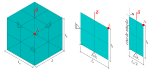
\includegraphics[scale = 1.0]{0701-Malha_ensaio_triaxial.pdf}
	\end{center}
	\caption{\label{malha_ensaio_triaxial}Domínio e discretização de um ensaio triaxial com modelo 3D, EPD e AXI}
\end{figure}

Os valores dos parâmetros do modelo constitutivo adotado na análise foram $E = 403$MPa, $\nu = 0.39$,  superficief = 2, superficieg = 2, $\phi = 0, \psi = 0, c_i = 0,7, c_p = 1,3, c_r = 0,9, \bar \varepsilon^p_{I} = 0,010, \bar \varepsilon^p_{II} = 0,050, \bar \varepsilon^p_{r} = 0,07$, Dalg = 0. Os parâmetros de coesão e de deformação plástica equivalente das zonas de endurecimento e amolecimento são coletadas do gráfico do ensaio, tal como apresentado na \autoref{ensaio_triaxial_parametros}. O valor de duas vezes a coesão está no fato de que não está sendo considerado o ângulo de atrito e de dilatância, fazendo com que a superfície de plasticidade se reduza a de von-Mises. Nesse aspecto, a variação do volume não considera a dilatância durante a deformação plástica. A parte viscosa do modelo constitutivo é eliminada utilizando uma coesão alta. O resultado da análise pode ser visto na \autoref{ensaio_triaxial_solucao}.
 
\begin{figure}[H]
 	\begin{center}
 		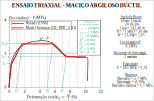
\includegraphics[scale = 0.9]{0702-ensaio triaxial argila ductil_coletando_parametros.pdf}
 	\end{center}
 	\caption{\label{ensaio_triaxial_parametros}Domínio e discretização de um ensaio triaxial com modelo 3D, EPD e AXI}
\end{figure}

\begin{figure}[H]
	\begin{center}
		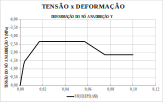
\includegraphics[scale = 1.0]{0703-ensaio triaxial argila ductil solucao.pdf}
	\end{center}
	\caption{\label{ensaio_triaxial_solucao}Resultado da análise para o ensaio triaxial}
\end{figure}

Como pode-se ver os valores deram exatamente iguais considerando 3D, EPD e AXI demonstrando que a implementação conseguiu essa generalidade. Caso o modelo seja de fato utilizado para estudos de túneis reais é sempre desejável ter ensaios triaxiais para fazer a validação ou eventuais calibrações nesse aspecto do modelo.

\section{Verificação da solução numérica com uma solução analítica considerando o endurecimento}

Essa verificação considerará uma das soluções analíticas deduzidas por \citeonline{Bernaud2020}. A solução analítica escolhida corresponde a um problema de um túnel profundo de seção circular sobre tensão geostática hidrostática com um critério de plasticidade de Tresca considerando endurecimento por deformação plástica, conforme \autoref{coesao_solucao_analitca_LAJSS}. 

\begin{figure}[H]
	\begin{center}
		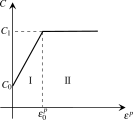
\includegraphics[scale = 1.2]{0704-lei de endurecimento ou amolecimento_coesao_solucao_analitca.pdf}
	\end{center}
	\caption{\label{coesao_solucao_analitca_LAJSS}Variação da coesão: I - trecho de endurecimento linear e II - comportamento perfeitamente plástico (adaptado de: \citeonline[p.  4]{Bernaud2020})}
\end{figure}
A expressão (\ref{eq:LAJSS1}) apresenta a solução analítica da convergência quando se adota $r=R_i$.
\begin{equation}
	\label{eq:LAJSS1}
	\dfrac{u(r)}{r} = \dfrac{(1-2\nu)(\nu+1)}{E}\left\{\sigma_x+\dfrac{2C_0}{1+2\dfrac{C'}{E'}}\left[\dfrac{C'}{E'}\left(\dfrac{1}{r^2}-\dfrac{1}{x^2}\right) y^2+\ln{\left(\dfrac{x}{r}\right)-\sigma_\infty} \right]  \right\}-\dfrac{2C_0}{E'}\left(\dfrac{y}{r}\right)^2
\end{equation}
em que $E'=E/(1+\nu), \nu, C' = (C_1-C_0)/\varepsilon_0^p$ são parâmetros do material. Essa solução é dependente também dos raios plásticos $x,~y$, da tensão na fronteira do raio plástico $\sigma_x$, das tensões geostáticas hidrostáticas $\sigma_\infty$ e da tensão no interior da cavidade do túnel $\sigma_i$. O restante das expressões para aplicar essa solução são:
\begin{equation} \label{eq:LAJSS2}
	{{\sigma }_{x}}=2{{C}_{1}}\ln \left( \frac{{{R}_{i}}}{x} \right)+{{\sigma }_{i}},~~~ 	{{x}^{2}}=\frac{2{{C}_{0}}}{E'\varepsilon _{0}^{p}+2{{C}_{1}}}{{y}^{2}}, ~~~ 	{{y}^{2}}=\frac{{{R}_{i}}}{{{\omega }_{0}}}{{e}^{\frac{({{\omega }_{1}}+{{\omega }_{2}}+{{\omega }_{3}})}{{{C}_{1}}}}} 
\end{equation}
\begin{equation} \label{eq:LAJSS3}
	{{\omega }_{0}}=\frac{2{{C}_{0}}}{E'\varepsilon _{0}^{p}+2{{C}_{1}}}, ~~~ 	{{\omega }_{1}}={{\sigma }_{i}}-{{\sigma }_{\infty }}-{{C}_{0}} , ~~~ {{\omega }_{2}}=\frac{{{C}_{0}}}{1+2\frac{C'}{E'}}\ln ({{\omega }_{0}}), ~~~ 	{{\omega }_{3}}=\frac{\frac{C'}{E'}\left[ 2({{C}_{0}}-{{C}_{1}})-\varepsilon _{0}^{p} \right]}{1+2\frac{C'}{E'}}
\end{equation}

Utilizando $Ri=1$m, $E=1430$MPa, $\nu = 0.4$, $C_0=0.21$MPa, $C_1=0.56$MPa, $\varepsilon _{0}^{p}=0.024$, $P_i = -\sigma_i = 2.5$MPa, $ P_\infty = -\sigma_\infty = 4.5$MPa tem-se, pela expressão analítica, $U_i(\%) = 5.91$. A Figura \autoref{solucao_numérica_LAJSS} apresenta a concordância do resultado numérico com um erro menor que 1\%.

\begin{figure}[H]
	\begin{center}
		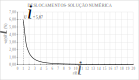
\includegraphics[scale = 1.0]{0705-lei de endurecimento ou amolecimento_coesao_solucao_numerica.pdf}
	\end{center}
	\caption{\label{solucao_numérica_LAJSS}Solução numérica considerando elastoplasticidade com endurecimento}
\end{figure}
Para essa solução numérica foi utilizado domínio em EPD (\autoref{malhaEPD_tunel}) e a relação (\ref{eq:ctr_cvm}) que considera a superfície de von-Mises inscrita em Tresca e as mesmas considerações para particularizar o modelo elastoplástico-viscoplástico para elastoplástico, ou seja, a parte viscosa do modelo constitutivo é novamente eliminada utilizando uma coesão alta. Para representar a mesma lei de endurecimento tem-se $c_i = 0.21\sqrt{3}/2$, $c_p = 0.56\sqrt{3}/2$, $c_r = 0.56\sqrt{3}/2, \bar \varepsilon^p_{I} = 0,024, \bar \varepsilon^p_{II} = 0,024, \bar \varepsilon^p_{r} = 0,024$. 

\section{Verificação do modelo Axissimétrico}
O modelo axissimétrico, apesar de estar limitado às condições de axissimetria, é um dos modelos mais importantes, pois considera o processo de escavação e colocação do revestimento de forma realista e permite fazer estudos paramétricos de forma mais eficiente que o modelo tridimensional. Aqui nesse capítulo será apresentado algumas verificações da solução considerando cada lei constitutiva separada: I - elásticidade, II - elastoplasticidade, III - viscoplasticidade e IV - elastoplasticidade-viscoplasticidade. Para o caso I, II e IV sem revestimento é possível verificar com soluções analíticas. Quando se tem revestimento a verificação tem de ser com outro \textit{software}, que nesse caso, será o GEOMEC91. O GEOMEC91 é um programa de elementos finitos para geomecânica para análises bidimensionais em axissimetria. Ele foi desenvolvido por \citeonline{Bernaud1991} e vem sendo utilizado em diversas dissertações e teses no PPGEC.

\subsection{Verificações do modelo axissimétrico em elasticidade}

O modelo constitutivo acoplado, por ser geral, tem que ser capaz de reproduzir o resultado em elasticidade colocando coesões elevadas na parte plástica e viscosa. Considerando $E =$1000MPa e 5000MPa, $\nu =$ 0.498MPa, $p_v = p_h = 5$MPa tem-se os resultados da \autoref{ELAST-D0-E1000-ER0-P5} e \autoref{ELAST-D0-E5000-ER0-P5}. As curvas cinzas são os perfis de convergência a cada passo de escavação e a vermelha no último passo. A curva verde pontilhada é a solução analítica.

\begin{figure}[H]
	\begin{center}
		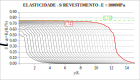
\includegraphics[scale = 1.0]{0706-AXI-SREVESTIMENTO-E1000.pdf}
	\end{center}
	\caption{\label{ELAST-D0-E1000-ER0-P5}Verificação solução numérica em elasticidade sem revestimento - E = 1000MPa}
\end{figure}

\begin{figure}[H]
	\begin{center}
		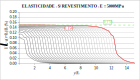
\includegraphics[scale = 1.0]{0707-AXI-SREVESTIMENTO-E5000.pdf}
	\end{center}
	\caption{\label{ELAST-D0-E5000-ER0-P5}Verificação solução numérica em elasticidade sem revestimento - E = 5000MPa}
\end{figure}

Cabe salientar que a mesma solução é obtida escavando todos os passos de uma única vez. Contudo, quando se tem revestimento não há solução analítica, pois ocorre a iteração entre o revestimento e o maciço. Para essa verificação é comparado o resultado do ANSYS com o GEOMEC91. A \autoref{ELAST-D0-E1000-ER30000-P5} mostra essa comparação considerando $E$ = 1000MPa com um revestimento de $Er$=30000MPa e $\nu$ = 0.3. Nesse caso, foi considerado um $d0$ = 0.

\begin{figure}[H]
	\begin{center}
		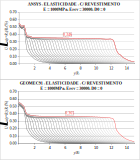
\includegraphics[scale = 1.0]{0708-AXI-SREVESTIMENTO-E1000-ER30000-D0.pdf}
	\end{center}
	\caption{\label{ELAST-D0-E1000-ER30000-P5}Verificação solução numérica em elasticidade com revestimento - $E$ = 1000MPa, $E_{rev}$ = 30000MPa, $d0$ = 0}
\end{figure}

O perfil de convergência apresenta um pico nas primeiras escavações, uma vez que na primeira escavação é escavado 3$l_p$. De qualquer forma, em comparação com a \autoref{ELAST-D0-E1000-ER0-P5} consegue-se ver que o revestimento tem um grande efeito sobre as deformações. Contudo, não é só o módulo de elasticidade do revestimento que conta, mas tão importante quanto, o d0. Considerando um $d_0=4l_p$ tem-se os resultados da \autoref{ELAST-D4-E1000-ER30000-P5}.

\begin{figure}[H]
	\begin{center}
		\includegraphics[scale = 1.0]{0709-AXI-SREVESTIMENTO-E1000-ER30000-D4.pdf}
	\end{center}
	\caption{\label{ELAST-D4-E1000-ER30000-P5}Verificação solução numérica em elasticidade com revestimento - $E$ = 1000MPa, $E_{rev}$ = 30000MPa, $d0$ = 4$l_p$}
\end{figure}

Na \autoref{ELAST-D4-E1000-ER30000-P5} pode-se ver pequenas ondulações no perfil de convergências do GEOMEC91 que não estão presentes no resultado do ANSYS. Essa diferença ocorre devido ao elemento finito utilizado. No GEOMEC91 é utilizado um elmento quadrático enquanto que no ANSYS linear.

Os gráficos apresentados aqui são extraídos do modelo axissimétrico. Contudo, as mesmas verificações foram feitas com o modelo tridimensional considerando a seção circular. Praticamente os mesmos resultados foram obtidos.

Como pode-se notar o modelo em elementos finitos com o modelo constitutivo acoplado conseguiu em elasticidade reproduzir outras soluções independentes. Ademais, a verificação do modelo em elasticidade foi muito importante para conferir se as escavações e a colocação do revestimento estavam sendo feitas corretamente. Além disso, deram uma ideia inicial da qualidade da malha.

\subsection{Verificações do modelo axissimétrico em elastoplasticidade}

De forma análoga à elasticidade, o modelo constitutivo acoplado, por ser geral, tem que ser capaz de reproduzir o resultado em elastoplasticidade colocando uma coesão viscoplástica elevada. Considerando $E =$1000MPa, $\nu =$ 0.498MPa, $p_v = p_h = 4$MPa, $c_i=c_p=c_r = \sqrt{3}/2$MPa e $3\sqrt{3}/2$MPa  tem-se os resultados da \autoref{PLAST-D0-E1000-ER0-P4-C1} e \autoref{PLAST-D0-E1000-ER0-P4-C3}. As curvas cinzas são os perfis de convergência a cada passo de escavação e a vermelha no último passo. A curva verde pontilhada é a solução analítica.

\begin{figure}[H]
	\begin{center}
		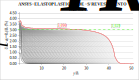
\includegraphics[scale = 1.0]{0710-AXI-PLAST-SREVESTIMENTO-D0-E1000-ER0-P4-C1.pdf}
	\end{center}
	\caption{\label{PLAST-D0-E1000-ER0-P4-C1}Verificação solução numérica em elasticidade com revestimento - $E$ = 1000MPa,  $c_i=c_p=c_r = \sqrt{3}/2$MPa}
\end{figure}
No caso em que $c_i=c_p=c_r = \sqrt{3}/2$MPa, foi necessário aumentar o número de passos de escavação $n_p = 128$ para que o patamar no perfil de convergência se desenvolvesse plenamente. A solução analítica é dada para esse patamar sem a influência da face de escavação ou das bordas do modelo.
\begin{figure}[H]
	\begin{center}
		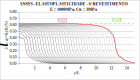
\includegraphics[scale = 1]{0711-AXI-PLAST-SREVESTIMENTO-D0-E1000-ER0-P4-C3.pdf}
	\end{center}
	\caption{\label{PLAST-D0-E1000-ER0-P4-C3}Verificação solução numérica em elasticidade com revestimento - $E$ = 1000MPa, $c_i=c_p=c_r = 3\sqrt{3}/2$MPa}
\end{figure}
 A próxima verificação, compreende a plasticidade dependente da pressão e não associada. Para tanto é utilizado um ângulo de atrito $\phi$=15$^\circ$ e um ângulo de dilatância $\psi$=0$^\circ$. O resultado pode ser visto na \autoref{PLAST-D0-E1000-ER0-P4-C1-KP15-KB1}. Essa solução apenas não converge quando se utiliza Newton-Raphson Completo com o módulo constitutivo consistente. Se for utilizar o módulo constitutivo consistente é necessário utilizar o Newton-Raphson Completo Assimétrico. A opção em que é utilizado Newton-Raphson Completo mas sem atualizar o módulo constitutivo converge para a solução. Outro aspecto importante, comparando o resultado da \autoref{PLAST-D0-E1000-ER0-P4-C1-KP15-KB1} com a \ref{PLAST-D0-E1000-ER0-P4-C1} é a sensibilidade com que a convergência é afetada pelo ângulo de atrito.
\begin{figure}[H]
	\begin{center}
		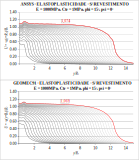
\includegraphics[scale = 1]{0712-AXI-PLAST--D0-E1000-ER0-P4-C1-KP15-KB1.pdf}
	\end{center}
	\caption{\label{PLAST-D0-E1000-ER0-P4-C1-KP15-KB1}Verificação solução numérica elastoplasticidade sem revestimento $E$ = 1000MPa, $c_i=c_p=c_r = \sqrt{3}/2$MPa, $\phi$=15$^\circ$ e $\psi$=0$^\circ$}
\end{figure}

A verificação da solução considerando a colocação de um revestimento com $E_{rev} = 30000$MPa, $\nu = 0.3$ e $d_0$=0 pode ser vista na \ref{PLAST-D0-E1000-ER30000-P4-C1}.

\begin{figure}[H]
	\begin{center}
		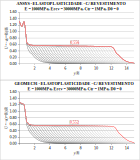
\includegraphics[scale = 1.0]{0713-PLAST-D0-E1000-ER30000-P4-C1.pdf}
	\end{center}
	\caption{\label{PLAST-D0-E1000-ER30000-P4-C1}Verificação solução numérica em elastoplasticidade com revestimento - $E$ = 1000MPa, $E_{rev}$ = 30000MPa, $c_i=c_p=c_r=\sqrt{3}/2$}
\end{figure}

\subsection{Verificações do modelo axissimétrico em viscoplasticidade}

De forma análoga à elasticidade e à elastoplasticidade, o modelo constitutivo acoplado, por ser geral, tem que ser capaz de reproduzir o resultado viscoplástico colocando coesões elevadas na parte elastoplástica. 

\subsection{Verificações do modelo axissimétrico em elastoplasticidade-viscoplasticidade}